\documentclass[MTech]{iitmdiss}

\usepackage{times}
\usepackage{epsf}
\usepackage{threeparttable}
\usepackage{setspace}
\usepackage{amsmath}
\usepackage{gensymb}
\usepackage{amsthm}
\usepackage{txfonts,pxfonts,amsfonts}
\usepackage{epsfig}
\usepackage{caption}
\usepackage{subcaption}
\usepackage{graphicx}
% \usepackage[square,numbers,sort]{natbib}
\usepackage[square]{natbib}
\usepackage{hyperref} % hyperlinks for references.
%\usepackage{algorithmic}
%\usepackage{algorithm}


%\include{commands}
\newcommand{\plt}{thesis_plots}
% Strut macros for skipping spaces above and below text in tables. 
\def\abovestrut#1{\rule[0in]{0in}{#1}\ignorespaces}
\def\belowstrut#1{\rule[-#1]{0in}{#1}\ignorespaces}

\def\abovespace{\abovestrut{0.20in }}
\def\aroundspace{\abovestrut{0.20in}\belowstrut{0.10in}}
\def\belowspace{\belowstrut{0.10in}}
%%%%%%%%%%%%%%%%%%%%%%%%%


\def\thesistitle{Motivic analysis of neuronal responses to visual stimuli}
\def\thesisauthor{Athul Vijayan}


\begin{document}
\bibliographystyle{iitm}
%%%%%%%%%%%%%%%%%%%%%%%%%%%%%%%%%%%%%%%%%%%%%%%%%%%%%%%%%%%%%%%%%%%%%% 
% Title page

\title{\thesistitle}

\author{\thesisauthor}

\date{April 2016}
\department{Engineering Design}

%\nocite{*}
\begin{singlespace}
\maketitle 
\end{singlespace} 



%%%%%%%%%%%%%%%%%%%%%%%%%%%%%%%%%%%%%%%%%%%%%%%%%%%%%%%%%%%%%%%%%%%%%%
% Certificate
\certificate

\vspace*{0.5in}

\noindent This is to certify that the thesis entitled {\bf {\thesistitle}}, 
submitted by {\bf {\thesisauthor}}, to the Indian Institute of Technology, 
Madras, for the award of the degree of {\bf Master of Technology}, 
is a bona fide record of the research work carried out by him under my
supervision. The contents of this thesis, in full or in parts, have not been
submitted to any other Institute or University for the award of any degree or
diploma.

\vspace*{1.4in}
\hspace*{-0.25in}
\begin{singlespace}
\noindent {\bf Dr.~Hema~A.~Murthy } \\
\noindent Research Guide \\ 
\noindent Assistant Professor \\
\noindent Dept. of Computer Science and Engineering\\
\noindent IIT-Madras, 600 036 \\
\end{singlespace}
\vspace*{0.20in}
\noindent Place: Chennai\\ 
Date:

%%%%%%%%%%%%%%%%%%%%%%%%%%%%%%%%%%%%%%%%%%%%%%%%%%%%%%%%%%%%%%%%%%%%%%
% Acknowledgements
\acknowledgements

**I would like to thank everyone who helped me.

%%%%%%%%%%%%%%%%%%%%%%%%%%%%%%%%%%%%%%%%%%%%%%%%%%%%%%%%%%%%%%%%%%%%%%
% Abstract
\abstract
\noindent KEYWORDS: \hspace*{0.5em} \parbox[t]{4.4in}{Markov Decision Processes,
Symmetries, Abstraction}
\vspace*{24pt}

\pagebreak
%%%%%%%%%%%%%%%%%%%%%%%%%%%%%%%%%%%%%%%%%%%%%%%%%%%%%%%%%%%%%%%%%%%%%%
% Table of contents etc.

\begin{singlespace}
\tableofcontents
\thispagestyle{empty}

\listoftables
\addcontentsline{toc}{chapter}{LIST OF TABLES}
\listoffigures
\addcontentsline{toc}{chapter}{LIST OF FIGURES}
\end{singlespace}


%%%%%%%%%%%%%%%%%%%%%%%%%%%%%%%%%%%%%%%%%%%%%%%%%%%%%%%%%%%%%%%%%%%%%%
% Abbreviations
\abbreviations
 
\noindent 
\begin{tabbing}
xxxxxxxxxxx \= xxxxxxxxxxxxxxxxxxxxxxxxxxxxxxxxxxxxxxxxxxxxxxxx \kill
\textbf{RLCS}   \> Rough Longest Common Subsequence \\
\textbf{LCSS}   \> Longest Common Segment Set \\
\end{tabbing}

\pagebreak

%%%%%%%%%%%%%%%%%%%%%%%%%%%%%%%%%%%%%%%%%%%%%%%%%%%%%%%%%%%%%%%%%%%%%%
%Notation

\chapter*{\centerline{NOTATION}}
\addcontentsline{toc}{chapter}{NOTATION}

\begin{singlespace}
\begin{tabbing}
xxxxxxxxxxx \= xxxxxxxxxxxxxxxxxxxxxxxxxxxxxxxxxxxxxxxxxxxxxxxx \kill
\textbf{$\rho(a, b)$}  \> Pearson correlation between $a$ and $b$\\
\textbf{V1}  \> Primary Visual Cortex\\
\end{tabbing}
\end{singlespace}
 
 \pagebreak
 \clearpage

\pagenumbering{arabic}


%%%%%%%%%%%%%%%%%%%%%%%%%%%%%%%%%%%%%%%%%%%%%%%%%%%%%%%%%%%%%%%%%%%%%%
\chapter{Introduction}
\label{chap:intro}

%%%%%%%%%%%%%%%%%%%%%%%%%%%%%%%%%%%%%%%%%%%%%%%%%%%%%%%%%%%%%%%%%%%%%%
\chapter{Background and Previous work}
\label{chap:lit}
\section{Visual pathway in brain} % (fold)
\label{sec:visual_pathway_in_brain}

% section visual_pathway_in_brain (end)
\section{Experiment setup} % (fold)
\label{sec:experiment_setup}
\subsection{Sinusoidal grating visual stimuli} % (fold)
\label{sub:sinusoidal_grating_visual_stimuli}

% subsection sinusoidal_grating_visual_stimuli (end)

\subsection{Natural videos visual stimuli} % (fold)
\label{sub:natural_videos_visual_stimuli}

% subsection natural_videos_visual_stimuli (end)
% section experiment_setup (end)

\section{Orientation and Directional selectivity of neurons in V1} % (fold)
\label{sec:orientation_and_directional_selectivity_of_neurons_in_v1}

% section orientation_and_directional_selectivity_of_neurons_in_v1 (end)

%%%%%%%%%%%%%%%%%%%%%%%%%%%%%%%%%%%%%%%%%%%%%%%%%%%%%%%%%%%%%%%%%%%%%%
\chapter{Analyzing neuronal properties}
\label{chap:searchmotif}
Characteristics of neurons in the V1 are discussed in the background section. In this chapter, we use experimental data to demonstrate the claimed properties of neurons in V1. In the experiment, a drifting sinusoidal grating video is shown to awake mice and neuronal responses were recorded. See Section~\ref{sub:sinusoidal_grating_visual_stimuli} for detailed experiment setup. 

Average response of a neuron is modeled as a function of orientation using a Gaussian function. Similarly, average response to various directions are modeled using a mixture of Gaussian functions. Root mean square of residuals are used as a goodness of fit measure.

Neurons in V1 are classified into simple, complex and unselective cells. Classifying a neuron into either of this class is useful as we can find the population of similar cells in the brain. Rather than thresholding OSI and DSI, We have used a k-means clustering algorithm with more features to classify cells.
\section{Quantifying Orientation and Directional selectivity} % (fold)
\label{sec:quantifying_orientation_and_directional_selectivity}
Modern imaging technologies allow examining responses of neurons with clarity. 
% section quantifying_orientation_and_directional_selectivity (end)

\section{Modeling neuronal response} % (fold)
\label{sec:modeling_neuronal_response_to_sinusoidal_gratings_stimuli}
Modeling the response of neuron to various orientations and visualizing is a great way to see if in fact there is a orientation selectivity. If the cell seems selective, we can characterize the degree of selectivity and preferred orientation.

Orientation tuning curve is modeled using a Gaussian function with constant offset. The empirical form of the orientation tuning curve is,
$$R_o(\theta) = C + R_p \exp\left\{\frac{-||\theta-\theta_{pref}||^2}{2\sigma^2}\right\}$$
Where $R_o(\theta)$ is the time-averaged response of neuron to angle of orientation $\theta$. Parameter $\theta_{pref}$ is the preferred orientation of the neuron. Tuning width $\sigma$  tell us how much the cell is selective. $C$ is a constant offset.

Similarly, we can model direction tuning curve using a mixture of Gaussian functions with a constant offset. 
$$R_d(\theta) = C + R_p \exp\left\{\frac{-||\theta-\theta_{pref}||^2}{2\sigma_1^2}\right\} + R_n \exp\left\{\frac{-||\theta-\theta_{null}||^2}{2\sigma_2^2}\right\}$$
Where $R_o(\theta)$ is the time-averaged response of neuron to angle of direction $\theta$. Relative magnitude of tuning widths, $\sigma_1$ and $\sigma_2$ denote the amount of directional selectivity. $C$ is a constant offset.
% section modeling_neuronal_response_to_sinusoidal_gratings_stimuli (end)

Parameters are estimated by minimizing squared sum of error. Sum of squared error is defined as:
$$SSE = \sum_{i=1}^N ||R(\theta_i) - R_o(\theta_i)||^2$$
A gradient descent algorithm finds the optimum parameters by minimizing SSE.
In Figure~\ref{fig:curvefit_complex} , fit of tuning curves of a complex cell is given. The distinct peak in the orientation tuning curve shows selectivity to orientation $\theta_{pref}$. In the direction tuning curve, peaks of different magnitude shows one direction is more preferred than other.
\begin{figure}[h]
  \begin{subfigure}[b]{0.5\textwidth}
    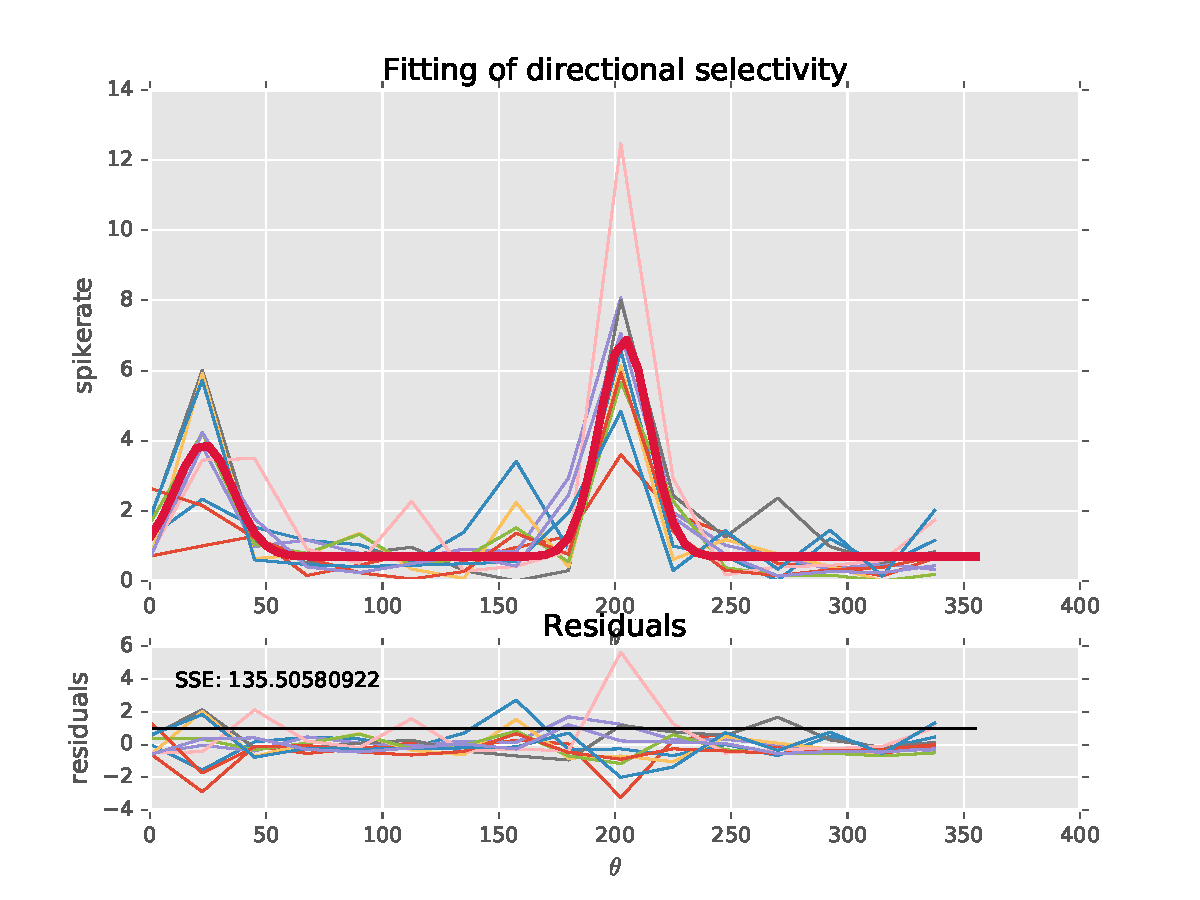
\includegraphics[width=\linewidth]{\plt/gratings_crvefit_n_3_2016_05_01_15_40_28.pdf}
    \caption{Orientation tuning curve}
    \label{fig:oritune_complex}
  \end{subfigure}%
  \begin{subfigure}[b]{0.5\textwidth}
    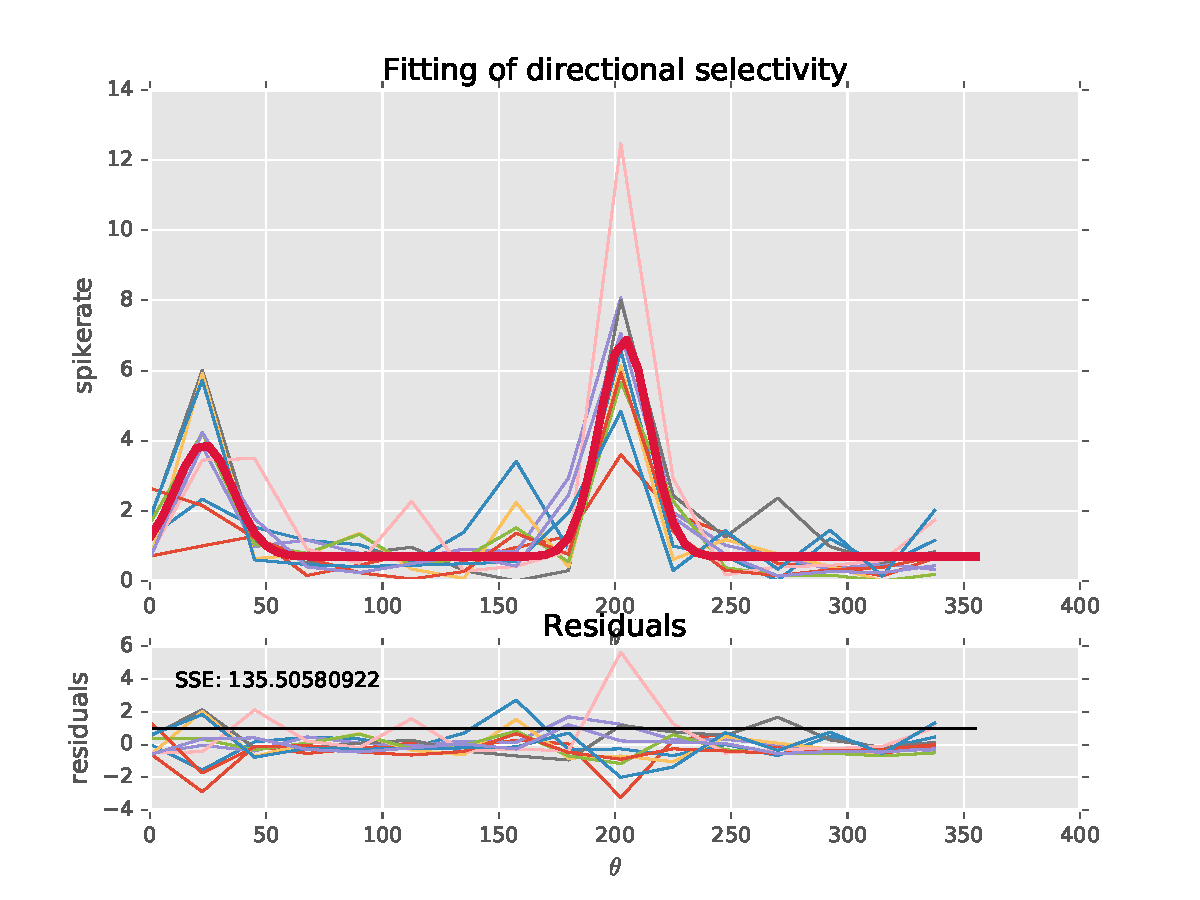
\includegraphics[width=\linewidth]{\plt/gratings_crvefit_n_3_2016_05_01_15_40_28.pdf}
    \caption{Direction tuning curve}
    \label{fig:dirtune_complex}
  \end{subfigure}%
  \caption{Fit of orientation and direction tuning curves of a neuron. The distinct peak in the orientation tuning curve shows selectivity to orientation $\theta_{pref}$. Different $\sigma_1$ and $\sigma_2$ in direction tuning curve shows direction sensitive cell. - Thus a complex cell}\label{fig:curvefit_complex}
\end{figure}

In Figure~\ref{fig:curvefit_simple} , fit of tuning curves of a complex cell is given. The distinct peak in the orientation tuning curve shows selectivity to orientation $\theta_{pref}$. In the direction tuning curve, peaks of same magnitude shows direction is irrelevant.
\begin{figure}[h]
  \begin{subfigure}[b]{0.5\textwidth}
    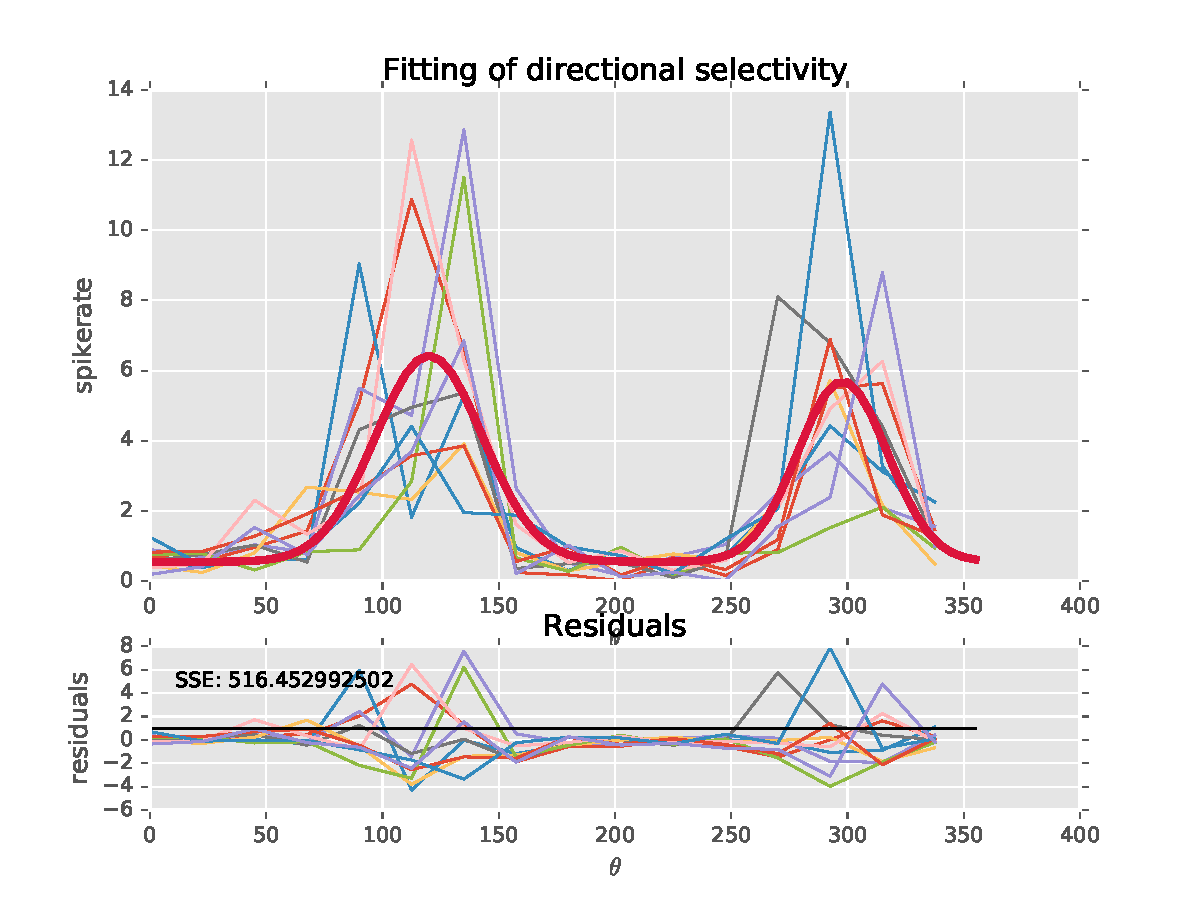
\includegraphics[width=\linewidth]{\plt/gratings_crvefit_n_0_2016_05_01_15_40_26.pdf}
    \caption{Orientation tuning curve}
    \label{fig:oritune_simple}
  \end{subfigure}%
  \begin{subfigure}[b]{0.5\textwidth}
    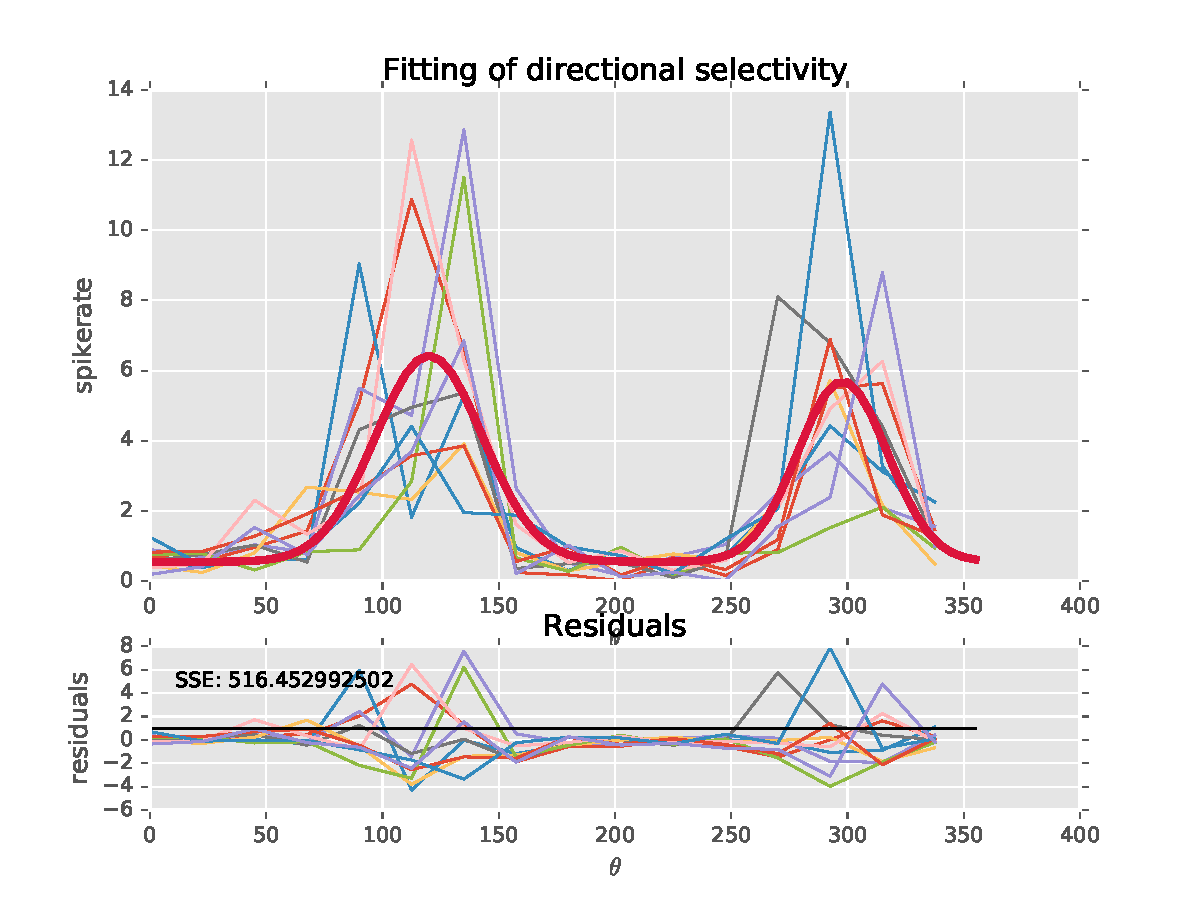
\includegraphics[width=\linewidth]{\plt/gratings_crvefit_n_0_2016_05_01_15_40_26.pdf}
    \caption{Direction tuning curve}
    \label{fig:dirtune_simple}
  \end{subfigure}%
  \caption{Fit of orientation and direction tuning curves of a neuron. The distinct peak in the orientation tuning curve shows selectivity to orientation $\theta_{pref}$. Similar $\sigma_1$ and $\sigma_2$ in direction tuning curve direction is irrelevant. - Thus a simple cell}\label{fig:curvefit_simple}
\end{figure}
\section{Classification of neurons based on selectivity} % (fold)
\label{sec:classification_of_neurons_based_on_selectivity}

% section classification_of_neurons_based_on_selectivity (end)
%%%%%%%%%%%%%%%%%%%%%%%%%%%%%%%%%%%%%%%%%%%%%%%%%%%%%%%%%%%%%%%%%%%%%%
\chapter{Searching for Motifs}
\label{chap:searchmotif}

%%%%%%%%%%%%%%%%%%%%%%%%%%%%%%%%%%%%%%%%%%%%%%%%%%%%%%%%%%%%%%%%%%%%%%
\chapter{Rough Longest Common Subsequence}
\label{chap:rlcs}

%%%%%%%%%%%%%%%%%%%%%%%%%%%%%%%%%%%%%%%%%%%%%%%%%%%%%%%%%%%%%%%%%%%%%%
\chapter{Inferences and Future work}
\label{chap:summary}

%%%%%%%%%%%%%%%%%%%%%%%%%%%%%%%%%%%%%%%%%%%%%%%%%%%%%%%%%%%%%%%%%%%%%%
\appendix
\chapter{Neural visual pathway}

%%%%%%%%%%%%%%%%%%%%%%%%%%%%%%%%%%%%%%%%%%%%%%%%%%%%%%%%%%%%%%%%%%%%%%
% Bibliography.
\pagebreak
\begin{singlespace}
  \begin{small}
	\bibliography{refs}
  \end{small}
\end{singlespace}
%%%%%%%%%%%%%%%%%%%%%%%%%%%%%%%%%%%%%%%%%%%%%%%%%%%%%%%%%%%%%%%%%%%%%%
\end{document}
